\section{Introduction}
\label{introduction}
\label{sec:intro}

\begin{figure}[tb]
\centering
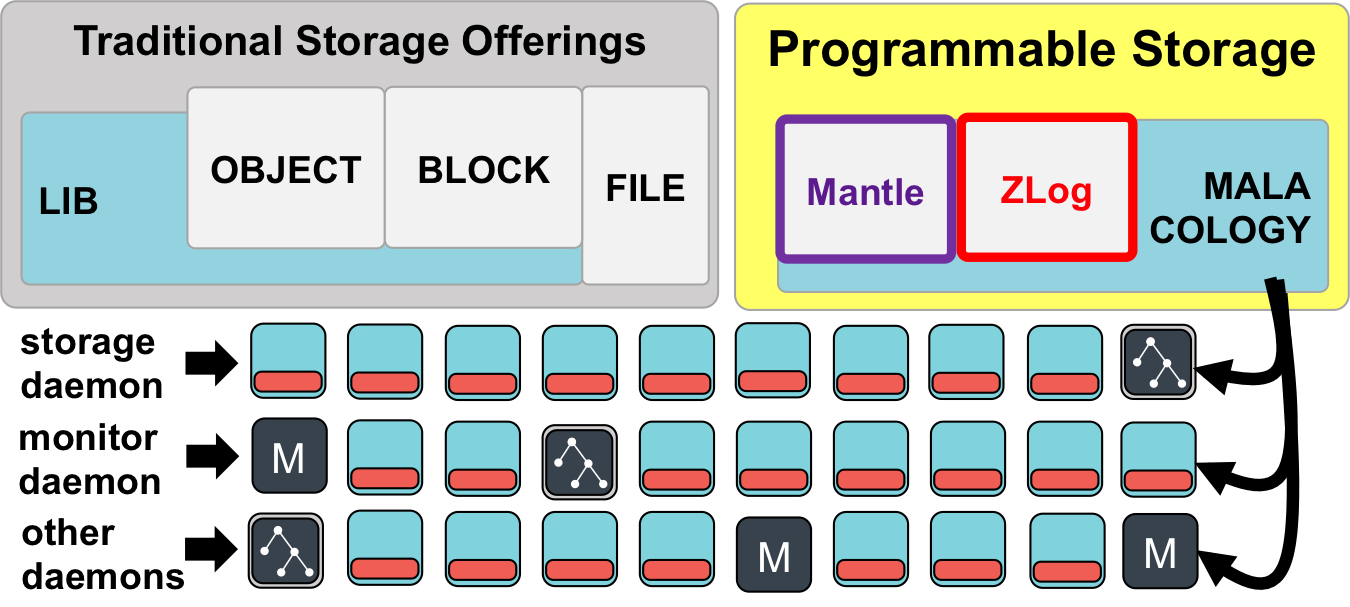
\includegraphics{figures/overview.png}
\caption{Scalable storage systems have storage daemons which store data,
monitor daemons (M) that maintain cluster state, and service-specific daemons
(e.g., file system metadata servers). Malacology enables the programmability of
internal abstractions (bold arrows) to re-use and compose existing subsystems.
With Malacology, we built new higher-level services, ZLog and Mantle, that sit
alongside traditional user-facing APIs (file, block,
object).}\label{fig:overview}
\end{figure}

A{\let\thefootnote\relax\footnote{$^{\dag}$ These authors contributed equally to
this work.}} storage system implements abstractions designed to persistently
store data and must exhibit a high level of correctness to prevent data loss.
Storage systems have evolved around storage devices that often were orders of
magnitude slower than CPU and memory, and therefore could dominate overall
performance if not used carefully. Over the last few decades members of the
storage systems community have developed clever strategies to meet correctness
requirements while somewhat hiding the latency of traditional storage
media~\cite{brewer_disks_2016}. To avoid lock-in by a particular vendor, users
of storage systems have preferred systems with highly standardized APIs and
lowest common denominator abstract data types such as blocks of bytes and byte
stream files~\cite{armbrust_view_2010}.

A number of recent developments have disrupted traditional storage systems.
First, the falling prices of flash storage and the availability of new types of
non-volatile memory that are orders of magnitude faster than traditional
spinning media are moving overall performance bottlenecks away from storage
devices to CPUs and networking, and pressure storage systems to shorten their
code paths and incorporate new
optimizations~\cite{gray_tape_2007,gray_flash_2008}.  Second, emerging ``big
data'' applications demand interface evolution to support flexible consistency
as well as flexible structured data
representations.~\cite{apache_contributors_parquet_2014}.  Finally,
production-quality scalable storage systems available as open source software
have established and are continuing to establish new, \emph{de-facto} API
standards at a faster pace than traditional standards
bodies~\cite{snia_implementing_2014,linux_foundation_kinetic_2015}.

The evolutionary pressure placed on storage systems by these trends raises the
question of whether there are principles that storage systems designers can
follow to evolve storage systems efficiently, without jeopardizing years of
code-hardening and performance optimization efforts.  In this paper we
investigate an approach that focuses on identifying and exposing existing
storage system resources, services, and abstractions that in a generalized form
can be used to \emph{program} new services. This `dirty-slate' approach of
factoring out useful code lets programmers re-use subsystems of the back-end
storage system, thus inheriting their optimizations, established correctness,
robustness, and efficiency. `Clean-slate' approaches could be implemented
faster but they do so at the expense of ``throwing away" proven code.

{\it \textbf{Contribution 1:}} We define a programmable storage system to be a
storage system that facilitates the re-use and extension of existing storage
abstractions provided by the underlying software stack, to enable the creation
of new services via composition.  A programmable storage system can be realized
by exposing existing functionality (such as \newcommentone{file system and
cluster} metadata services and synchronization and monitoring capabilities) as
interfaces that can be ``glued together'' in a variety of ways using a
high-level language. Programmable storage differs from \emph{active
storage}~\cite{riedel:vldb98}---the injection and execution of code within a
storage system or storage device---in that the former is applicable to any
component of the storage system, while the latter focuses at the data access
level. Given this contrast, we can say that active storage is an example of how
one internal component (the storage layer) is exposed in a programmable storage
system.  \addressesissue{4}

To illustrate the benefits and challenges of this approach we have designed and
evaluated Malacology, a programmable storage system that facilitates the
construction of new services by re-purposing existing subsystem abstractions of
the storage stack.  We build Malacology in Ceph, a popular open source software
storage stack.  We choose Ceph to demonstrate the concept of programmable
storage because it offers a broad spectrum of existing services, including
distributed locking and caching services provided by \newcommentone{file
system} metadata servers, durability and object interfaces provided by the
back-end object store, and propagation of consistent cluster state provided by
the monitoring service (see Figure~\ref{fig:overview}).  Malacology is
expressive enough to provide the functionality necessary for implementing new
services.  \addressesissue{4}

Malacology includes a set of interfaces that can be used as
building blocks for constructing novel storage abstractions, including:

\begin{enumerate}

\item An interface for managing strongly-consistent time-varying
\textbf{service metadata}.

\item An interface for installing and evolving domain-specific, cluster-wide
\textbf{data I/O} functionality.

\item An interface for managing access to \textbf{shared resources} using a
variety of optimization strategies.

\item An interface for \textbf{load balancing} resources across the cluster.

\item An interface for \textbf{durability} that persists policies using the
underlying storage stack's object store.

\end{enumerate}

{\it \textbf{Contribution 2:}} We implement two distributed services using
Malacology to demonstrate the feasibility of the programmable storage approach:

\begin{enumerate}

\item A high-performance distributed shared log service called ZLog, that is an
implementation of CORFU~\cite{balakrishnan_corfu_2012}

\item An implementation of Mantle, the programmable load balancing
service~\cite{sevilla:sc15-mantle}

\end{enumerate}

The remainder of this paper is structured as follows. First, we describe and
motivate the need for programmable storage by describing current practices in
the open source software community. Next we describe Malacology by presenting
the subsystems within the underlying storage system that we re-purpose, and
briefly describe how those system are used within Malacology
(Section~\ref{sec:malacology}).  Then we describe the services that we have
constructed in the Malacology framework (Section~\ref{sec:services}), and
evaluate our ideas within our prototype implementation
(Section~\ref{sec:evaluation}).  We conclude by discussing future and related
work.
